\documentclass{article}
\usepackage[margin=0.2cm,papersize={15cm,15cm}]{geometry}
\usepackage{amsmath,amssymb}
\usepackage{tikz}
\usetikzlibrary{arrows.meta,positioning,shapes.geometric}
\pagestyle{empty}

\definecolor{rank0Col}{RGB}{24, 100, 171}    % Deep Blue
\definecolor{rank1Col}{RGB}{43, 138, 62}     % Forest Green
\definecolor{rank2Col}{RGB}{217, 119, 6}     % Warm Amber
\definecolor{rank3Col}{RGB}{128, 43, 179}    % Royal Purple
\definecolor{arrowCol}{RGB}{224, 49, 49}     % Crimson Red
\definecolor{tokenGold}{RGB}{230, 135, 0}    % Gold Accent

\begin{document}
\centering
\vspace*{\fill}
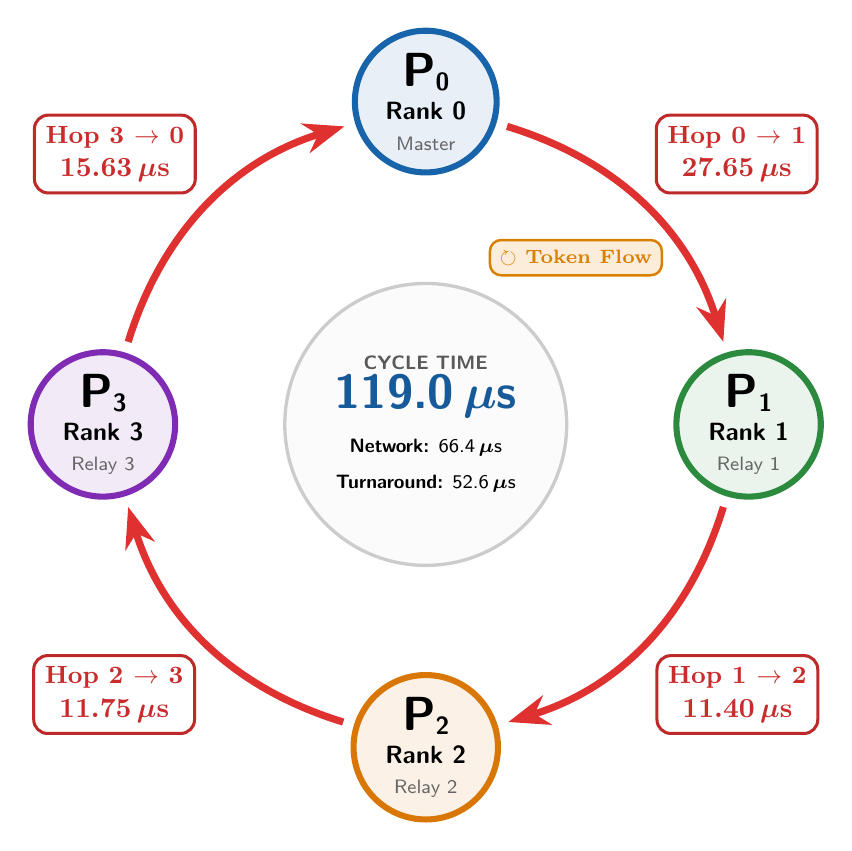
\begin{tikzpicture}[
    font=\sffamily,
    >=Stealth,
    % Process Node Style
    procNode/.style={
        circle,
        minimum size=1.80cm,
        line width=2.2pt,
        align=center,
        inner sep=2pt
    },
    % Hop Latency Badge Style - Crisp, high-contrast, zero overlap
    hopBadge/.style={
        rounded corners=5pt,
        draw=arrowCol!85!black,
        fill=white,
        line width=1.1pt,
        inner sep=4pt,
        align=center,
        font=\small,
        text=arrowCol!90!black
    },
    % Directed Ring Arrow Style
    ringArrow/.style={
        ->,
        line width=2.6pt,
        draw=arrowCol,
        shorten >=4pt,
        shorten <=4pt
    }
]

    % Ring Radius - generous clearance preventing any collisions
    \def\R{4.1cm}

    % Process Nodes placed on circle
    \node[procNode, draw=rank0Col, fill=rank0Col!10] (P0) at (90:\R) {
        {\textbf{\LARGE P\raisebox{-1.5pt}{\small 0}}}\\[0pt]
        {\small\textbf{Rank 0}}\\[-1pt]
        {\scriptsize\textcolor{black!60}{Master}}
    };

    \node[procNode, draw=rank1Col, fill=rank1Col!10] (P1) at (0:\R) {
        {\textbf{\LARGE P\raisebox{-1.5pt}{\small 1}}}\\[0pt]
        {\small\textbf{Rank 1}}\\[-1pt]
        {\scriptsize\textcolor{black!60}{Relay 1}}
    };

    \node[procNode, draw=rank2Col, fill=rank2Col!10] (P2) at (270:\R) {
        {\textbf{\LARGE P\raisebox{-1.5pt}{\small 2}}}\\[0pt]
        {\small\textbf{Rank 2}}\\[-1pt]
        {\scriptsize\textcolor{black!60}{Relay 2}}
    };

    \node[procNode, draw=rank3Col, fill=rank3Col!10] (P3) at (180:\R) {
        {\textbf{\LARGE P\raisebox{-1.5pt}{\small 3}}}\\[0pt]
        {\small\textbf{Rank 3}}\\[-1pt]
        {\scriptsize\textcolor{black!60}{Relay 3}}
    };

    % Clockwise Directed Arcs with Latency Badges outside the perimeter
    % P0 -> P1 (Top-Right quadrant)
    \draw[ringArrow] (P0) to[bend left=28] 
        node[midway, above right=6pt, hopBadge] {
            \textbf{Hop 0 $\to$ 1}\\[1pt]
            \textbf{\normalsize 27.65\,$\boldsymbol{\mu}$s}
        } (P1);

    % P1 -> P2 (Bottom-Right quadrant)
    \draw[ringArrow] (P1) to[bend left=28] 
        node[midway, below right=6pt, hopBadge] {
            \textbf{Hop 1 $\to$ 2}\\[1pt]
            \textbf{\normalsize 11.40\,$\boldsymbol{\mu}$s}
        } (P2);

    % P2 -> P3 (Bottom-Left quadrant)
    \draw[ringArrow] (P2) to[bend left=28] 
        node[midway, below left=6pt, hopBadge] {
            \textbf{Hop 2 $\to$ 3}\\[1pt]
            \textbf{\normalsize 11.75\,$\boldsymbol{\mu}$s}
        } (P3);

    % P3 -> P0 (Top-Left quadrant)
    \draw[ringArrow] (P3) to[bend left=28] 
        node[midway, above left=6pt, hopBadge] {
            \textbf{Hop 3 $\to$ 0}\\[1pt]
            \textbf{\normalsize 15.63\,$\boldsymbol{\mu}$s}
        } (P0);

    % Center Circular Summary Hub (Compact, round, perfectly isolated)
    \node[
        circle,
        draw=gray!40,
        fill=gray!3,
        line width=1.2pt,
        align=center,
        inner sep=7pt
    ] at (0, 0) {
        \textcolor{gray!70!black}{\scriptsize\bfseries CYCLE TIME}\\[2pt]
        {\bfseries\LARGE\textcolor{rank0Col!90!black}{119.0\,$\boldsymbol{\mu}$s}}\\[4pt]
        \scriptsize\textbf{Network:} 66.4\,$\boldsymbol{\mu}$s\\[1pt]
        \scriptsize\textbf{Turnaround:} 52.6\,$\boldsymbol{\mu}$s
    };

    % Token Flow Direction Indicator (Centered cleanly in upper-right quadrant)
    \node[
        rounded corners=4pt,
        draw=tokenGold!95!black,
        fill=tokenGold!15,
        line width=0.9pt,
        inner sep=3.5pt,
        font=\scriptsize\bfseries,
        text=tokenGold!95!black
    ] at (48:2.85cm) {$\circlearrowright$ Token Flow};

\end{tikzpicture}
\vspace*{\fill}
\end{document}
